%You can delete all the comments after you have finished your document
%this sets up the defaults for the documents, 12pt font and A4 size. The article type sets this up as such as opposed to letter or memo.

%for the finer points LaTeX see https://en.wikibooks.org/wiki/LaTeX or http://tex.stackexchange.com/

\documentclass[12pt,a4paper]{article}
\usepackage{titlesec} %these are how we import packages, one helps set up footers and title layout
\usepackage{fancyhdr}
\usepackage{titlesec}
\newcommand{\sectionbreak}{\clearpage}
\usepackage{apacite}
% !TEX TS-program = pdflatex
% !TEX encoding = UTF-8 Unicode
\usepackage[utf8]{inputenc} % set input encoding (not needed with XeLaTeX)
\usepackage{graphicx} % support the \includegraphics command and options
\graphicspath{{figures/}}
% \usepackage[parfill]{parskip} % Activate to begin paragraphs with an empty line rather than an indent

%%% PACKAGES
\usepackage{booktabs} % for much better looking tables
\usepackage{array} % for better arrays (eg matrices) in maths
\usepackage{paralist} % very flexible & customisable lists (eg. enumerate/itemize, etc.)
\usepackage{verbatim} % adds environment for commenting out blocks of text & for better verbatim
\usepackage{subfig} % make it possible to include more than one captioned figure/table in a single float
\usepackage[toc,page]{appendix}
% These packages are all incorporated in the memoir class to one degree or another...
\usepackage{algorithm}
\usepackage{algpseudocode}
\algdef{SE}[LOOP]{Loop}{EndLoop}[1]{\algorithmicloop\ #1}{\algorithmicend\ \algorithmicloop}%


%header and footer settings
\pagestyle{fancyplain}
\fancyhf{}
\renewcommand{\headrulewidth}{0.5pt}
\renewcommand{\footrulewidth}{0.5pt}
\setlength{\headheight}{15pt}
\fancyhead[L]{Matthew Lenathen - 40506678}
\fancyhead[R]{ SOC10101 Honours Project}
\fancyfoot[L]{}
\fancyfoot[C]{\thepage}

%this starts the document
\begin{document}

%you can import other documents into your main one, these layout the Title and Declarations on its own page.
%you might need to change these to \ if your on Microsoft Windows.
\newcommand{\HRule}{\rule{\linewidth}{0.5mm}}

\begin{titlepage}
	\begin{center}

	\HRule \\[0.4cm]
    	{\Large \bfseries Real-Time Cloth Simulation using Extended Position Based Dynamics\par}
	\vspace{0.2cm}
	\HRule \\[1.5cm]

	
    	\vspace{3cm}
	\begin{minipage}{0.4\textwidth}
	\begin{center} \large
        \emph{}\\
        	Matthew Lenathen - 40506678
				
   	 \end{center}
    	\end{minipage}
	
	\vspace{2cm}
    	\begin{minipage}{1\textwidth}
    	\begin{center} \large
        
		Submitted in partial fulfilment of \\
		the requirements of Edinburgh Napier University \\
		for the Degree of \\
        	BSc (Hons) Games Development
    	\end{center}
    	\end{minipage}

    	\vfill

    	% Bottom of the page
	\begin{minipage}{1\textwidth}
    	\begin{center} \large
		School of Computing
    	\end{center}
    	\end{minipage}
	
	\vspace{1cm}
    	{\large \today}


	\end{center}
\end{titlepage}
%{\large Submitted in partial fulfilment of the requirements of Edinburgh Napier University for the Degree of }

\section*{Authorship Declaration}
\vspace{0.5cm}
\begin{flushleft}
I, Matthew Lenathen, confirm that this dissertation and the work presented in it are my own achievement.\newline

Where I have consulted the published work of others this is always clearly attributed;\newline

Where I have quoted from the work of others the source is always given. With the exception of such quotations this dissertation is entirely my own work;\newline

I have acknowledged all main sources of help; \newline

If my research follows on from previous work or is part of a larger collaborative research project I have made clear exactly what was done by others and what I have contributed myself;\newline

I have read and understand the penalties associated with Academic Misconduct.\newline

I also confirm that I have obtained informed consent from all people I have involved in the work in this dissertation following the School's ethical guidelines.\newline
\end{flushleft}

\begin{flushleft} \large
\emph{Signed:} \\
\end{flushleft}

\vspace{.5cm}

\begin{flushleft} \large
\emph{Date:} 
\\
\end{flushleft}

\vspace{.5cm}

\begin{flushleft} \large
\emph{Matriculation no: } 40506678  \\
\end{flushleft}
\pagebreak

\section*{General Data Protection Regulation Declaration}
\vspace{0.5cm}
\begin{flushleft}
Under the General Data Protection Regulation (GDPR) (EU) 2016/679, the University cannot disclose your grade to an unauthorised person. However, other students benefit from studying dissertations that have their grades attached. \newline

\vspace{0.5cm}

Please sign your name below one of the options below to state your preference.\newline
\vspace{0.5cm}

The University may make this dissertation, with indicative grade, available to others.\newline
\vspace{3cm}
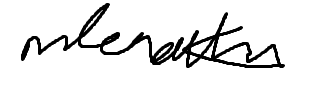
\includegraphics[height=2\baselineskip]{figures/sig.png}

The University may make this dissertation available to others, but the grade may not be disclosed.\newline
\vspace{3cm}


The University may not make this dissertation available to others.\newline
\end{flushleft}



\pagebreak

%LaTeX let you define the abstract separately so it wont get sucked into the main document.
\begin{abstract}
Abstract here
% fill the abstract in here
\end{abstract}
\pagebreak

\tableofcontents % is generated for you
\newpage

\listoftables
%generated in same way as figures
\newpage

\listoffigures
%you may have captions such as equations, listings etc they should all appear as required
%these are done for you as long as you use \begin{figure}[placement settings] .. bla bla ... \end{figure}
\newpage

\section*{Acknowledgements}
Insert acknowledgements here
\subsection*{}
	I would like to thank my cat, dog and family.
\newpage

\section{Introduction}
\newpage
\section{Literature Review}
\subsection{Introduction to Cloth Simulation}
Cloth is a major aspect of realistic simulations. Present in many different industries such as: film, games development and virtual reality, cloth simulation is a challenge that combines maths, physics and programming. \\

Cloth simulation is a subsection of Physics-based animation. PBA uses physics and code to create a plausible looking display of realistic effects, e.g. fluid simulations, soft-body dynamics etc. Cloth is defined as a flexible plane of some material or fabric that can move in unique ways, such as bending or stretching. This makes it a tricky and unique problem to simulate accurately. \\

The end goal of a cloth simulation can vary depending on the intended use. In computer graphics, physical accuracy is not the highest priority, the end product is mostly focused on how it looks. This is in contrast to cloth simulations for real-world engineering problems, their focus being primarily on physical accuracy, in order to help them predict real-world scenarios. Real time usage of cloth is also very important in the games industry, and will be discussed later. \\

As it is featured in such a wide range of fields, the literature relating to cloth is plentiful. In this section, many papers, books and articles will be discussed and compared in order to give context to the focus of this project, Extended position based dynamics (XPBD).

\subsection{Brief History of Cloth Simulation}
\label{History}
Cloth simulation is a very active field in research, and has been for a handful of decades. The first graphic models used to mimicking cloth was developed in 1986 by Jerry Weil. Before this, cloth objects were created by mapping textures onto rigid surfaces. His method represents cloth as a 2d grid of 3d coordinates, and focused on simulating cloth held at constraint points, like a draped fabric. \cite{weil_synthesis_1986}. This method didn't allow for cloth movement but it piqued the interest of the graphics community regarding cloth simulation. \\

An important development was made in 1987 by Terzopoulos et al. Their method was a general solution for representing elastic deformable objects like rubber or paper. This method is physically-based, meaning the object is active and can respond to external forces such as gravity or wind. Their paper presented various equations on how objects such as cloth or paper should deform when presented with forces, it also describes how they integrated these equations through time, which is a key topic in simulation. This research laid the groundwork for many more physically based models, and more cloth oriented methods. \cite{terzopoulos1987elastically} \\

As time went on, more ways to simulate cloth were developed, such as particle based systems by Breen et al. in 1992. In particle-based systems, the simulating focused on a series of connected particles, and how they react with each other. The way these particles interacted formed the basis for the cloth dynamics. \cite{breen1992physically} In their paper they decided to move away from continuum based methods and switch towards a particle based model. In 1995, Provot developed a similar particle system but used point masses connected with springs to represent a cloth mesh. \cite{provot1995deformation} \\

In 1998, Baraff and Witkin developed a method that used implicit integration combined with the cloth being represented as a mesh of triangles. This new proposed system allowed for bigger time steps to be taken and faster simulation times. This system is still used today as the foundation for new methods. \cite{Baraff1998largesteps} \\

Later, in 2007, Müller et al. developed and published a paper on a state of the art method for dynamic simulations called Position Based Dynamics. This technique, along with a newer extended version, is the main focus of this project and will be discussed in a later chapter. \cite{muller2007position} and \cite{macklin2016xpbd}

\subsection{Underlying Physics}
\label{Physics}
In order to discuss the advancements and methods within the current literature, it is important to delve into the underlying physics that allow cloth simulations to function. This section will go over important principles that are crucial to creating such simulations.
\\

Often, cloth is represented by particles. These particles have position p, and velocity v, and can be arranged in a grid structure to model a piece of cloth. In order to represent the actual geometry of these particles, they can be arranged into triangles that make up a bigger mesh. When these triangles are small enough, that is when the simulated cloth can look realistic.
\\

For simulations such as mass-spring systems, forces are the primary mechanism for making the particles move. In this case, spring forces between two particles are calculated using Hooke's law, and they say that if the spring is stretched or compressed more than the springs rest length, forces are applied to remedy that. Other common forces are gravity and wind and these will be applied to near all simulations regardless of if it is a force-based method or not.
\\

As the main focus of this project is position-based dynamics, constraints must be discussed too. Constraints are pivotal to position-based dynamics because instead of relying on forces, PBD directly adjusts positions to satisfy constraints. Constraints can vary depending on the situation but usually there are some staples such as distance, bending and collision constraints. Each of these will ensure that the particles within the simulation act as realistic as possible. 


\subsection{Offline Cloth Simulation} 
Cloth simulation can generally by split into two categories: Offline and Real Time. Offline simulations are calculated, tweaked and edited before being rendered to the screen. Commonly used in film and animation, visual fidelity is of utmost importance. Offline calculations can also help in a real time scenario by precomputing effects. \\

\subsubsection{Fine Cloth Interactions}
As offline simulations are not limited by the time between each frame, they can afford to focus on realism. They can do this by scaling the number of triangles up and allowing for finer interactions like folding and wrinkling, these interactions being crucial to a convincing cloth simulation. A great example of such work is presented in a paper by Selle et al., they detail their method of creating a high resolution simulation with up to two million triangles, that can accurately capture the intricate details of cloth. \cite{4522545}\\

At the time of publication, cloth simulations were adding physically-based interactions like wrinkles through a separate modelling system. This can be seen in the work by Cutler et al., in which they created a system that allowed the artist to add in wrinkles on top of an existing character's clothing \cite{10.1145/1073368.1073384}. They achieved this by splitting it into stages: wrinkle creation and wrinkle evaluation. In the wrinkle creation phase, the artists use a tool to create winkle patterns, which get turned into a set of forces on the surface. Next, in the wrinkle evaluation phase, the system generates these deformations based on character poses, and the artists can either choose to keep these generated wrinkles, or alter the pattern until satisfactory results are achieved.\\
In their results, they were able to use their system to create clothing wrinkles on hundreds of characters for a feature-length animated film. They noted that in production, close to zero hand-tweaking was needed for the wrinkles, proving its reliability.\\
When discussing their work, they did note that the visual results from a dynamic clothing simulation is much preferred to what they achieved with their kinematic wrinkle system. This is where the work of Selle et al., aims to improve upon. \\

In their paper, they aimed to create a system where fine details such as folds and wrinkles were created in a physically-based fashion, from the various forces acting on the cloth. Their setup included a mass-spring system with edge and bending spring, and a modified time integration scheme. One notable contribution from their work is how they handle collisions. They note that in order to achieve high resolution folds and wrinkles, the self collisions and interactions must be extremely robust, as they are what cause cloth to create these effects in the first place. In their paper, they created a hybrid repulsion/collision technique that works based on the last known collision. They also utilise parallelism to further improve computing times.\\
In their initial evaluation, the researchers put their system to the test with a twisted cloth model comprising 500,000 triangles.  This example took an average of 30 minutes to calculate each frame. They found that their system was able to simulate an extremely detailed cloth with accurate folds and wrinkles, alongside realistic collision and repulsion. These advanced and realistic effects lend themselves to the offline nature of the simulation, as calculating all of these effects are extremely computationally expensive.

\subsubsection{Precomputing Cloth Effects}
In computer graphics, it is often said that precomputing everything is simply not viable due to how many interactions can occur, but in a paper by Kim et al., they discuss precomputing secondary cloth effects. \cite{kim2013near}. In this case, secondary cloth effects refer to things such as folds and wrinkles, these are expensive simulate in real-time. In this paper, they propose a method to use many thousand CPU-hours to calculate these advanced effects in advance, based on a character motion graph. They achieve this by representing a character with two motion graphs, the primary graph simply being the movement of the character, and the secondary being the cloth dynamics. \\

To evaluate their method, they acquired 12 unique motion clips for the primary graph, and used ARCSim cloth simulator for the cloth motion. They found that in their massive precomputation, they were able to generate good looking cloth animations for any random paths through the primary graph. Initially their secondary graph was just one to one mapping of character poses to cloth, but this proved insufficient for realistic motion, so the secondary graph was made much more complex. 
Overall, the inclusion of precomputing cloth motion, helped simulate incredibly detailed secondary features of cloth, such as wrinkles and folds. This research also links into game development in their discussion section, they propose that viewing a database of precomputed cloth motion could be a great benefit when creating games, as certain scenes could be viewed and edited, also bad looking cloth could be fixed by hand to help realism within the game. \\

In summary, it can be seen that offline simulations, compared to real-time, prioritise visual plausibility and realistic effects. These simulations can be achieved due to their non-real-time nature, being able to compute all necessary effects in advance, and being able to tweak things that don't quite match with others. Making offline simulations great for things such as: animation, fashion design and the film industry. This level of details contrasts with real-time simulations, where they must balance out visual quality with the demands of immediate computation.


\subsection{Real Time Cloth Simulation}
Real time cloth simulations are created by computing the cloth dynamics at runtime, allowing interaction with the user through input and changes from the environment. As the time between frames on real time applications is small, the dynamics need to be calculated and applied efficiently, usually on the GPU. The most common use case for real time cloth simulations are in video games, and as these games also have lots of other calculations going on in the background, means optimisation is even more important. This section will discuss the literature on methods to create these simulations and how they compare with each other. \\
\subsubsection{Mass-Spring Systems}
\label{Mass-Spring}
As mentioned in section \ref{Physics}, mass-spring systems are a popular approach to cloth simulations. They represent a cloth as a grid of particles that can exert forces on each other. The way they exert forces are through springs. The first example of this system, as noted in section \ref{History}, was introduced by Provot \cite{provot1995deformation}.\\

In his paper, he posited that the current state of cloth animation at the time had a lack of realism, especially in the realm of elasticity. His proposed mesh had three different types of springs to achieve different effects. Structural springs being the most basic, it connects adjacent particles in a grid formation. Shear springs connect particles diagonally, and bend springs connect particles by skipping a particle in between, e.g. connecting particle [i,j] to particle [i+2,j+2]. \\

This research successfully modelled a more realistic cloth using mass-springs and inspired research into more efficient mass-spring systems for use in real time, such as the work by Kang and Cho \cite{kang2012photorealistic}. It is known that the mass-spring model suffers from instability, especially at larger time steps, Kang and Cho aim to resolve this instability by proposing a more stable and accurate integration model. They note that an implicit integration scheme would help stabilise the system but it cannot be easily parallelised, so an improved explicit method was chosen. \\

It is noted that Hooke's law is commonly used with mass-spring systems to calculate forces, but Kang and Cho decided to use a harmonic oscillation model, allowing for integration.\\
With their new integration method and parallelism implemented, they were able to simulate cloth containing 16,384 particles and 161,544 springs at  over 68 frames per second. This shows that mass spring systems can be a good tool for simple simulations, although in their results they also show that once the springs get to a large size, in this case 1,200,000 springs, the frame rate drops to 15. It can be seen in current day simulations that the additional complexity from all the springs, stiffness tuning and overall accuracy lead to mass-spring systems not being the optimal method for real time cloth simulations.

\subsubsection{The Continuum Model}
While representing cloth with particles and springs can be straightforward and relatively pleasing to look at, there is a downside to this method, the real world representation of cloth. It is very hard to come up with a spring model that accurately represents various cloth materials such as nylon. This is where the continuum system for cloth fits in. The continuum method treats cloth as a continuous material made up of triangles rather than particles with space in-between, and instead of looking at spring forces, continuum looks at how each triangle is stretched and compressed. \\

As mentioned in section \ref{History}, Baraff and Witkin proposed one of the first continuum models in their paper \cite{Baraff1998largesteps}. A few others attempted such models such as \cite{terzopoulos1987elastically}. Although in their implementation, the damping forces weren't explored in much depth. Another paper by \cite{carignanclothy} built upon the work by Terzopoulos et al. and improved the damping forces by adding a force that damps cloth stretch and shear. They used an explicit integration scheme so was unfortunately limited by small time steps. These works lead Baraff and Witkin to develop their model. Their goal was to come up with a method that allows for larger time steps to be taken in simulation, as most at the time were bottlenecked by small time steps to remain stable. In their method, they employ an implicit integration scheme which allowed for much better performance, when combined with the simple formulation of internal forces. With this continuum representation, they were able to successfully model the common forces like shearing, bending and stretching. \\ 

In their results, they tested multiple setups including clothing. They found that changing the bend stiffness factor, didn't affect in running times a great deal, which explicit simulators wouldn't be able to do. They were also able to estimate their performance in terms of number of particles, and found that it was slightly better than \(O(n^{1.5})\) which was what they expected.\\

This paper laid the groundworks for many continuum implementations, one of which being a paper on data-driven elastic models for cloth simulation \cite{wangdatadriven}. Their goal was to more closely represent how different materials are simulated, ideally close to their real world counterpart. It does this by representing cloth with a piecewise linear elastic model. They explain that real world cloth items such as clothes often have anisotropic properties from the woven nature of cloth, and that this is often ignored by most cloth simulations for simplicity. A part of their research was a way to measure real life samples of cloth, construct a database of parameters are use them directly in their cloth simulation which was a very interesting way to get realistic results.
\\

Finite element analysis is a way to break down the cloth into discrete elements such as triangles, and the physical behaviour is calculated based on the material properties and forces acting on it. In 2020, Kim discussed how most cloth simulation are either made from finite element methods, position based dynamics or mass-spring systems, and that the Baraff-Witkin model doesn't really fit into these categories. In his paper he formulated a version of the Baraff-Witkin model but entirely in terms of finite elements \cite{FEMcantunderstand}. \\ 


\subsubsection{Cloth Simulation with Camera Capture}
As cloth simulation is such a wide field of research, there are many alternative methods and interesting papers to look at, one such idea is SimulCap by \cite{Yu_2019_CVPR}. SimulCap is a method of capturing human movement while also capturing dynamic details such as folds and wrinkles. It uses a RGBD (RGB depth) camera. Their problem with other recent implementations were the lack of realism, in part due to the human and cloth being considered as one piece of geometry, and also the results not being editable, which is a huge aspect of a lot of use cases, i.e. virtual dressing applications. So, for SimulCap, the authors decided to combine a layered representation of the human body, while also having a separate cloth simulation that matches the human movement. For their cloth simulation, they chose to use a mass-spring model for simplicity and also an explicit integration scheme with a small time step for stability. In their results, they compared their implementation with DoubleFusion, another previous system by \cite{yu2018doublefusion}, which is a state-of-the-art system for real time human capture. The authors found that SimulCap achieves a much more realistic cloth representation, mainly due to the separation of geometry as described earlier. The limitations of this system lie in the variation of clothing, e.g. thick jumpers remain challenging to simulate, also due to the simple nature of the cloth simulation, the realism could be improved upon by choosing a more advanced technique. \\

In a more recent paper by Wang et al., in 2023, they address the problem of extracting cloth movement combined with clothing motion, by proposing a novel method of capturing the human motion and clothing separately using double layer neural radiance fields (NeRF) \cite{Wang_2023_CVPR}. NeRF is a method of reconstructing a 3D scene using sparse 2D images. This is makes it a perfect method for cloth simulation using camera capture.During the optimisation phase, they introduce a physics-aware cloth simulation network to properly handle the cloth dynamics to ensure realism.

They comment on the previous implementation, SimulCap, by saying it failed to track the motion of the clothing to achieve editable clothing on humans, which is a prerequisite to most VR/AR apps. Their solution, using NeRFs, model both the body and the clothing in template space, which can then be transformed into observation space using deformation fields. Then, using the two NeRFs from before, the rendered images can be synthesized.

This approach addresses the problems with previous camera capture implementations. Its physics network is taught from simulation data, to constrain the clothing and ensure physically plausible clothing deformations.
In their comparison to state of the art methods, which include DeepCap and NerfCap, they found that their implementation vastly outperformed the other methods without a cloth template, and achieved a much higher accuracy during geometry tracking.


\subsubsection{Cloth Simulation with Neural Networks}
\label{neuralSection}
Another interest alternative method to cloth can be found in the research of \cite{neuralCloth}, a cloth simulation framework that uses an unsupervised deep learning methodology. This has been attempted in the past but the other approaches do not handle cloth dynamics. The authors note that while supervised learning systems have been used before, it requires huge volumes of data, and it has to be repeated for every garment/body, so they chose an unsupervised approach. For their cloth representation, they chose to use a particle based system that also considers external forces like wind and collision, this cloth is then skinned to a 3D model. After training their model, they compared their results to other unsupervised approaches such as \cite{bertiche2021pbns}. They evaluated their framework with multiple different body motions such as jumping and spinning. They found that their approach was the only one capable of achieving dynamic cloth effects. In terms of limitations, unsupervised learning compared to supervised takes much longer and is more computationally expensive, and neural cloth has yet to implement cloth self-collision which is a crucial component of most simulators.
\\

Another example of cloth simulations using neural networks can be found in the works of Oh et al., where they propose a hierarchical cloth simulation method that combines traditional physical based methods with deep neural networks (DNN) \cite{OhNeural}. They note that proper physically based cloth animation is expensive, so being able to utilise DNNs to replace the complex computation with data inferred from the network will reduce the cost significantly.

Their proposed method would split the simulation into two parts. Firstly, a low resolution or coarse model of the cloth is calculated using a normal physically based method. Then, the DNN is used to calculate the finer levels of the cloth, reducing the computation cost. They note that due to only calculating the coarsest level of cloth using a physically-based method, the overall cloth simulation won't be as accurate as a fully physically-based model but it successfully prevents errors stemming from the DNN, and guarantees a reliable simulation. This can be seen in Figure \ref{fig:DNN}.
\begin{figure}[h]
	\caption{An overview of how this implementation works}
	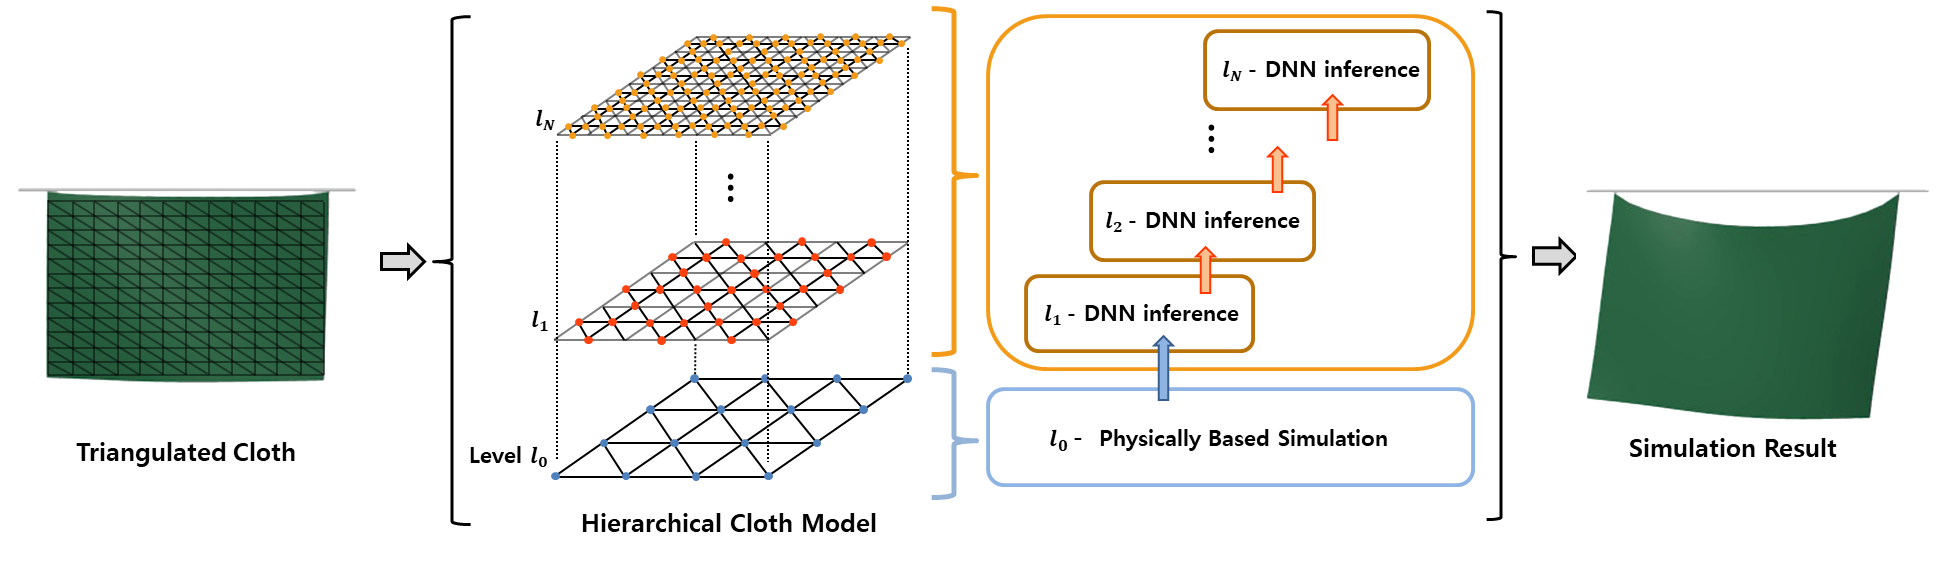
\includegraphics[width=\textwidth]{DNN.png}
	\label{fig:DNN}
\end{figure}

In their results, they constructed the simulation with three levels, one physically based used projective dynamics, and two DNN models. Projective dynamics will be covered in section \ref{otherMethods}. They compared time performance of their method against a normal implicit integration simulation, and against a projective dynamics implementation with an optimised algorithm applied to it called ADMM (alternating direction method of multipliers) \cite{ADMM}. They found that their hierarchical model that uses DNN improved performance, especially on configurations with many particles, e.g. flags and curtains. They do admit that the accuracy is not on the same level as completely physically based implementations but the results generated were of a high standard and were fast to generate. One final thing to note is that if the cloth is overstretched by external forces, the DNN can sometimes give unusual wrinkles near the bottom of the cloth. They aim to improve this in future work by updating the DNN model to also hold information such as velocity and momentum.


\subsubsection{Shape Matching}
Shape matching is a technique that allows an object to deform but tries to maintain the form of the original shape. In 2005, Müller et al., utilised shape matching to come up with a new method to simulate deformable objects \cite{ogshapematching}. It does this by replacing energies by geometric constraints, and forces by the distance of current positions to goal positions. These goal positions are determined by shape matching, given a rest state. They mention that because the points are always drawn to goal positions, the overshooting issue with explicit methods is completely removed.\\

In their algorithm, their idea is given a set of particles with an initial configuration, every time step the particles are moved towards their goal position, and these goal positions are determined by the original configuration of the shape. In terms of performance, it depends on the number of points used, and they note it is hard to compare it to another model such as mass-spring systems, as the technique depends on the number of clusters chosen, which cannot be reflected in the other models.\\
Overall, this shape matching approach to simulation provides an unconditionally stable simulation that is inexpensive to compute, although the model is not physically accurate.\\

This research inspired a paper on cloth simulation using shape matching in 2013 \cite{BENDER2013945}. As mentioned before, using shape matching for simulations proved unconditionally stable, so a model specifically designed for cloth simulation was created. They note that normal shape matching approaches that use regions, cannot differentiate between shearing, bending and stretching, which are crucial to represent cloth accurately. To combat that, they introduce a novel approach to use a multi-resolution model instead of region based. This can be seen in Figure \ref{fig:shape}, where a is a nested model that shares vertices between levels, and b is a non-nested model that do not share vertices. The results in this paper use a nested configuration. This multi-resolution model will allow for the simulation of fabrics that have different stretching/shearing stiffness. It is also noted that this method is fast due to it scaling linearly with the size of the cloth. \\

\begin{figure}[h]
	\caption{Two levels in a multi-resolution configuration, where a is a nested model and b is a non-nested model.}
	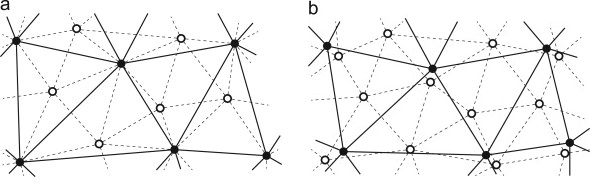
\includegraphics{shapeMatching.jpg}
	\label{fig:shape}
\end{figure} 
A shape matching approach that used regions was attempted before \cite{regionshapecloth}. But in this model, it introduces forces that influence the bending stiffness and depend on the size of the model, and this is undesirable in cloth simulation. Another problem is that due to small regions within a large model, high stretching and shearing stiffness cannot be obtained. This lead to the development of the multi-resolution approach.\\

In terms of performance, they simulated meshes between 10000 and 100000 triangles to test their scalability, and confirmed their linear relationship between computation time and number of triangles. They also implemented a GPU version of the method which resulted in a much faster compute time. They found in similar setups, the multi-resolution method was around 9 times faster than a standard mass-spring system, and around 15 times faster than a corotational finite element method, a method created by Etzmuss et al. \cite{etzmuss2003fast}. Overall, the multi-resolution approach provided a very noticeable speed-up compared to other approaches, at the cost of physical accuracy.
\\

Another implementation of shape matching was proposed by Vassilev, using shape matching to improve upon a traditional mass-spring model \cite{shapeMatchingMassSpring}. Once shape matching is applied, the springs no longer follow Hooke's law but the stability of the simulation is much improved at larger time steps. At the base, this model is based on the work of Provot, discussed in section \ref{Mass-Spring} \cite{provot1995deformation}. The modification made is replacing Hooke's law with shape matching. Vassilev was inspired by the work of Müller et al, in their original shape matching paper, but instead of shape matching on regions of vertices, Vassilev used it on springs. Each mass connected by one spring will have its own goal position to try to achieve. \\
After implementing it in OpenGL with compute shaders, the implementation was tested on a human figure wearing jeans, to monitor the stability of the shape matching springs. He found that for low time steps, the number of iterations that the shape matching method took to stitch the jeans was roughly the same or slightly higher than the original mass spring model. Since the original model is not stable for time steps above 40ms, the shape matching implementation proved better for larger time steps.

Overall, he found that the shape matching spring implementation was considerably more stable and was less dependant on time steps than the original mass spring system. He proposed this method could be used in real time simulation for things such as trying on clothes on models.

\subsubsection{Position Based Dynamics}
A great number of techniques discussed above have been force based, and these forces are used to calculate accelerations. Finally these accelerations are integrated to find the velocities and positions of particles. The Position based dynamics (PBD) technique takes a unique approach to physically based animations by omitting the velocity layer and directly working on the positions of particles. \cite{muller2007position} The main advantage is the controllability, the integration instability discussed in section \ref{Mass-Spring} is completely avoided due to the lack of explicit integration. As this is a real time technique, it is greatly suited to games development, as it is very helpful to have direct control over positions of objects within the game.\\

It was noted that even though PBD was the first fully position based approach, there had been other attempts to utilize positions in this way, such as \cite{fisixArticle}. In his approach, Jacobsen manipulated the positions directly using a Verlet integrator. The authors mention that Jacobsen didn't go into depth in terms of constraints, which is crucial in cloth simulation. PBD aims to improve upon it by giving a general approach to constraints.\\

To fully discuss the technique, the algorithm must be analysed. In the algorithm, an object is represented by N vertices and M constraints. The vertices are the particles which have mass m, position x and veloctiy v. The constraints contain a few more properties: cardinality, a function, set of indices, stiffness and a type of either equality or inequality. It is noted that the equality property is satisfied if the function of that constraint is equal to 0, and likewise if it has type inequality, it is satisfied if the function is more than equal to zero. The stiffness affects the strength of the constraints and it ranges from 0 to 1.

\begin{algorithm}
\caption{Position Based Dynamics Algorithm}
\begin{algorithmic}[1]
\ForAll{vertices $i$}
	\State initialize $x_i = x_i^0$, $v_i = v_i^0$, $w_i = 1/m_i$
\EndFor
\Loop
	\ForAll{vertices $i$}\State $v_i \leftarrow v_i + \Delta t w_i f_{ext}(x_i)$
	\EndFor
	\State dampVelocities$(v_1, \dots, v_N)$
	\ForAll{vertices $i$}
		\State $p_i \leftarrow x_i + \Delta t v_i$
	\EndFor
	\ForAll{vertices $i$}
		\State generateCollisionConstraints$(x_i \rightarrow p_i)$
	\EndFor
	\Loop{solverIterations \textbf{times}}
	\State projectConstraints$(C_1, \ldots, C_{M+M_{coll}}, p_1, \ldots, p_N)$
	\EndLoop
	\ForAll{vertices $i$}
		\State $v_i \leftarrow (p_i - x_i) / \Delta t$
		\State $x_i \leftarrow p_i$
	\EndFor
	\State velocityUpdate$(v_1, \dots, v_N)$
\EndLoop
\end{algorithmic}
\end{algorithm}
\newpage
Now it can be broken down to see what each part does. Lines 1 to 3 is just initialising each particle with initial position, velocity and inverse mass. Line 6 is where external forces get added to the system, Müller et al. notes that if gravity is the only external force then the line becomes $v_i \leftarrow v_i + \Delta tg$ where g is the gravitational acceleration. Next, on line 10, the new positions are estimated with a explicit Euler integration step, they are then adjusted in the line 15 loop as many times as needed until all constraints are satisfied. Once completed, the line 18 loop then moves the positions to the calculated position and updates the velocity. 
\\
This algorithm can be classed as unconditionally stable as the integration method in lines 19 and 20 do not use future positions/velocities, but instead calculate physically possible configurations and move the vertices to them.\\

In the paper, the authors also discuss their implementation of a cloth simulator for use in games. Their simulator accepts a triangle mesh and creates two constraints, stretching and bending constraints. Much like the springs in mass-spring systems, these constraints force the positions of the particles to satisfy them in order to continue the simulation, this relates to the loop in line 15 of the algorithm.
\\
To test their cloth simulation, they integrated the method into a game environment and conducted various experiments. They note that a positive to this method is that their bending and stretching terms are independent which can lead to more results when testing values. \\ 
In one of their tests they used one way coupling to link cloth to a stationary object, and two way coupled the bottom of the cloth to a rigid body, it resulted in realistic twisting and swaying, but more importantly ran at more than 380fps which showcases the efficiency of this method. \\
They were also able to test tearing of the cloth. Their tearing process is as follows: when an edge stretches past a threshold value then it is split, with the triangles above being assigned to the original vertex and the lower triangles assigned to the duplicate. They claim this is also extremely stable.\\

Overall, this paper was a very interesting approach to cloth simulation at the time, and influenced a great deal of work into real time cloth, eventually being used in Nvidia's physX software which in turn is used very frequently in game development.

\paragraph{Extended Position Based Dynamics} \mbox{} \\
In 2016, Müller collaborated with Miles Macklin and Nuttapong Chentanez to extend position based dynamics and improve upon the original method \cite{macklin2016xpbd}. Their problems with the original stemmed with iteration count and time step affecting the stiffness of the simulated object, specifically: constraints become stiff as iteration count increases/time step decreases. This effect is discussed in the 2014 survey on position-based methods \cite{bender2014survey}. \\
Their solution to this problem involved creating a new constraint formulation that corresponds to elastic potential energy. It also introduces a total Lagrange multiplier, which is a technique used to find the local maxima and minima of a function that is subject to constraints, e.g. in cloth this could be a distance constraint. This Lagrange multiplier allows the constraints to be solved irrespective of time step.\\

To test this on cloth, they set up the same cloth configuration for PBD and XPBD and compared them. They found that PBD became progressively stiffer as the iteration count increased but XPBD remained consistent. They also found a small downside of XPBD in terms of performance per-iteration, but this was less than 2\% of total simulation time. \\

In the limitations, the authors note that the method is only an approximation of an implicit Euler integrator, but this still creates very realistic real time results. Even so, if the application requires great accuracy, it would be advisable to choose a more traditional simulation method.

\label{otherMethods}
\paragraph{Other PBD methods} \mbox{} \\
\label{t}
In 2012, Kim et al., tackled a problem that all cloth has to deal with: inextensibility \cite{longrange}. At the time, existing methods had to solve non-linear systems which are computationally expensive. The authors proposed a new method, long range attachments (LRA). It is designed with the fact that in computer games, cloth is typically attached to the kinematic body of whatever is wearing the cloth. It uses this to create a constraint and enforce global inextensibility. This method can be applied to existing physics methods such as position based dynamics.\\

This works by creating a constraint on a fixed point, e.g. the part of cape attached to a characters shoulders. It then computes the distance from this particle to other attached particles. If a particle goes beyond a certain radius it is projected back towards the surface of a sphere with the centre of that sphere being the attachment point.
\\

The time taken to handle these LRA constraints scales linearly with the number of attachment points. This can be used to optimise the simulation by pruning certain attachment points. For example, in their cape test, they only choose the closest attachment point to each particle and it shows good results. It gets tricky when working on other shapes and for each configuration, it is recommended to find certain groups of pinned points, e.g. a waistline for a skirt.
\\

In their results, they found that the implementation provided a efficient and simple way to solve the stretching problem of cloth in games. They note that this method is only applicable to cloth applied to characters such as dresses, skirts and capes and that any environmental cloth such as a tissue or paper would see no benefit.
\\

Another interesting approach to position based dynamics is found in the works of Bouaziz et al. \cite{projectivedynamics}. They worked on bridging the gap between position based dynamics, a fast physically inaccurate method, and finite element methods. This lead to robust and efficient implementation that was accurate and supported many different types of constraints. Since continuum methods have the unfortunate side effect of being considerable more expensive than other methods, it would be beneficial to have the accuracy of finite element methods with the efficiency of position based dynamics, this is what projective dynamics aims for. The way they achieve this is by instead of using typical constraints found in position based dynamics, they use constraints derived from continuous deformation energies. With this method they can also perform a local and global optimisation step, meaning that for each element, they project it onto the constraint goal, and at the end the global step combines all of these and finds a compromise. 

This is similar to shape matching, which the authors note. \cite{ogshapematching}. Except in shape matching, the constraint projections are used to create the elastic forces instead of potentials.

When comparing this implementation to PBD, the authors note that the stiffness due to time step problem in the original PBD is solved due to including a momentum term. So that the cloth can behave in a similar way no matter the chosen time step.

When analysing the results, they test a cloth setup as a flag on a pole, which can be seen in Figure \ref{fig:pd}. They used edge constraints and external wind force to simulate movement. They were able to simulate the flag tearing in high wind by removing edge constraints when the strain on the cloth exceeds a certain limit.
\\

\begin{figure}
	\centering
	\caption{The simulation remaining stable in high wind speeds}
	\includegraphics[scale=0.5]{PDFlag.png}
	\label{fig:pd}
\end{figure}

In 2022, Li et al., proposed a new differentiable cloth simulation based on projective dynamics, but with dry frictional contact to simulate cloth self collision \cite{diffCloth}. The key difference of this work is that the simulation is differentiable, meaning gradients can be computed through backpropagation. This means that it can utilise many optimisation methods that result in a great speedup compared to non differentiable simulations. It also aims to  further improve upon the physical accuracy of projective dynamics by adding dry frictional contact. The paper showcases the simulator in many different use cases to showcase the efficacy of it.
\\
One of these examples showcases the usefulness of dry frictional contact, a piece of cloth falling onto a sphere. This is a very standard test in cloth simulation. This example contains both self collision from the cloth and also external contact with the sphere. After colliding the motion was mostly from the frictional component.
\\

Another example is a real-to-sim implementation of a flag. They used real motion of a flag blowing in the wind and tried to create a digital simulation copy. This was particularly tricky as it involved estimating what material was used and also modelling the wind condition at the time. They found it to be a good recreation of it but noted that due to the final loss function being non-zero, it was still imperfect. This is most likely due to the simplistic wind model they employed and could be improved with a more sophisticated model, such as one from a neural network.
\\

When evaluating the implementation, they found that it successfully accommodated rich and detailed self contact, differentiability and dry frictional contact. Since it was differentiable, they were able to utilise backpropagation and observe a significant speedup when compared to other direct solvers. There are a few limitations with this model, one being that since it is based on projective dynamics, it limits the choice of material. Another significant drawback is that the solver doesn't guarantee convergence, even though it is rare for this to happen, it still results in a costly switch to a direct solver. They note that they hope to resolve this in the future.

\subsection{Future Trends}
Since clothing is so prevalent in daily life, the graphics and physics research communities are always striving to improve and innovate the simulation of cloth. The evolution of cloth simulation can and will take many paths. One such path can be seen recently in the works of Clegg et al., which is robot-assisted dressing \cite{robot}. In the future, robots will most likely be interacting physically with humans more, one of these areas could be robot-assisted dressing. As clothing is extremely dynamic, the robot will need accurate cloth simulations to properly assist dressing.
\\

Another possible future trend would be cloth simulations with AI. As previously discussed in section \ref{neuralSection}, there are already examples of cloth simulations using neural networks for constraints. As machine learning and AI techniques improve, we could see more models being trained on real world clothing data and being used in more simulations.
\\

Finally, one more possible future trend is the increasing realism of clothing simulations. As seen in section \ref{t}, projective dynamics utilised the high accuracy of continuum based methods to more accurately simulate clothing. Perhaps in the future, continuum models will improve to accurately simulate a massive range of materials and textures that all have different properties. This would impact most use cases of cloth simulation such as garment try ons, video games and more.
\subsection{Conclusion}
The field of cloth simulation has faced major advancements in the past two decades through a variety of approaches both traditional and novel. Both offline and real-time simulations have seen great improvements through the evolution of methods and by building upon previous works. 
\\

Offline simulation has seen advancements in the form of accuracy and attention to detail. As these simulations are not bound by frame times, they can afford to spend much more time computing effects. This leads to simulations with incredible precision. These are typically seen in animation and film for high visual fidelity.
\\

Real time simulations have also seen big improvements to how they are made. As the use cases for clothing simulations are so large, there have been many different methods to creating simulations, such as camera capture. This is an important step forward as it enables the capture of real life clothing which not only helps to create realistic simulations, but can also be used as data to be fed into other computational models.
\\

Neural networks have also been a big focus for many researchers in the field due to the rapid improvement of AI techniques in recent years. These neural networks can have great predictive capabilities and room to learn off of previous data, which makes it suitable for large or detailed cloth models. Neural network cloth simulations will continue to be improved upon with models holding more data and variables, resulting in more physically accurate simulations.
\\

Despite all of these advancements, the field continues to face hurdles in developing these simulations, such as scalability, computational efficiency and physical accuracy. The future of cloth simulations will likely be solving these problems and discovering new techniques to more accurately model cloth as it appears in the real world.
\\

In conclusion, the literature on cloth simulation reflects a massive field, that is marked by novel and innovate approaches dedicated to improving the realism of cloth simulation. The combination of traditional methods rooted in classical physics, and the interesting techniques in computer science such as neural networks and camera capture highlights the progress of the field to date, but also opens the door to future breakthroughs that will further improve and scale cloth simulations.
\newpage



\section{Rest of Diss}

\subsubsection{Overview Of Project Content and Milestones}

This is a sub sub section with a list of bullet points.
\begin{itemize}\itemsep0pt
	\item A working X, that will be used for this investigation.
	\item Investigation of current tools and their potential use during an investigation of X .
	\item Programming of X with related frameworks Y and Z.
	\item That is all.
\end{itemize}


\section{Chapter 2}
The following bibliographic information on Writing a literature review is contained in the \emph{bibliography.bib} file 
The template automatically starts new chapters on a new page.  The associated guidelines tell you what the available styles do and also how to structure a report.
There is a section break on this page that you should be careful NOT to delete otherwise the references and appendices will be numbered continuously with the rest of the document.

% another example section
\section{Additional Information / Knowledge Required}
Experience with Linux and managing Virtual machines, networking.
So on and so forth...


\bibliographystyle{apacite}
\bibliography{bibliography}

%you can crate this on a extra tex document just like the title or any other part of the document.
\newpage
\begin{appendices}
\section{Project Overview}
%insert IPO

\begin{subappendices}
\subsection{Example sub appendices}
...
\end{subappendices}

\section{Second Formal Review Output}
Insert a copy of the project review form you were given at the end of the review by the second marker

\section{Diary Sheets (or other project management evidence)}
Insert diary sheets here together with any project management plan you have

\section{Appendix 4 and following}
insert content here and for each of the other appendices, the title may be just on a page by itself, the pages of the appendices are not numbered, unless an included document such as a user manual or design document is itself pager numbered.
\end{appendices}

\end{document}
